\chapter{Evaluation}
\label{chapter:evaluation}
This chapter will introduce the results that have been achieved through the implementation and experiments. Section~\ref{section:specificationrequirements} describes whether all the specifications as defined in~\ref{subsection:representation} have been met. Section~\ref{section:experiments_evaluation} presents the results of the two experiments that have been performed.

\section{Specification requirements}
\label{section:specificationrequirements}
In section~\ref{subsection:representation}, we drafted a set of specifications to which the new user interface must comply. These specifications enforce that all required functionality is implemented, and thus we will now evaluate if all specifications have been met.

\todo{je kunt dat woord "specification" toch wel weghalen in die tabel steeds}
\begin{table}[H]
	\center

	\begin{tabularx}{\textwidth}{llX}
		\toprule
		Specification ID		&	Requirements met		& Justification \\
		\midrule
		Specification S1		& Yes								& The \texttt{menus} and \texttt{menu} commands can always be called \\
		Specification S2		& Yes								& The \texttt{get} command allows the user to access an object\\
		Specification S2-A	& Yes								& The \texttt{properties} command lists an object's properties. If a property is an object, that object can be accessed.\\
		Specification S3		& Yes								& The \texttt{get} command allows the user to access a collection. Parented collections can be accessed with the \texttt{collections} command.\\
		Specification S4		& Yes								& The \texttt{action} command allows the user to invoke an action. \\
		Specification S4-A	& Yes								& If an action has parameters, the user is prompted to provide them. \\
		Specification S5		& Yes								& The \texttt{help} command opens a help menu with context-specific commands explained. \\
		Specification S6		& Yes								& The \texttt{quit} command logs the user out. \\
		Specification S7		& Yes								& The \texttt{errorService} manages error handling. \\
		\bottomrule
	\end{tabularx}
	
	\caption{Evaluation of the specifications}
	\label{table:specificationevaluation}
		
\end{table}

Since all specifications have been succesfully implemented, we can confirm that the integrity of the domain model has been maintained in our new user interface. Together with our findings in section~\ref{subsection:performancedifference} we will use these results to answer research question~\ref{RQ2}.

\section{Experiments}
\label{section:experiments_evaluation}
This section presents the results of our two experiments. Both experiments were focused on a set of five scenarios. These scenarios describe short tasks on which we have performed \acrshort{goms} analysis in the context of both user interfaces, as outlined in section~\ref{subsection:goms_evaluation}, and in addition the tasks were executed by test subjects in timed experiments. The results of the timed experiments are shown in section~\ref{subsection:timetrial_evaluation}.

The following scenarios have been used in our experiments:
\todo{Heel mooi, dit overzicht!}
\begin{table}[H]
	\center
	
	\begin{tabularx}{\textwidth}{lX}
		\toprule
		Scenario		&	Description \\
		\midrule
		Scenario 1	& Create a new Contact with the following details: \newline
								- Name: Sander Ginn \newline
								- Company: Eurocommercial \newline
								- Mobile number: +31 6252 5983 \newline
								- Email: sander@ginn.it \newline \\
		Scenario 2	& 	- Go to contact 'Clarisse Bentz' \newline
								- Add her to the contact group 'Management Board' with a new role 'Secretary' \newline \\
		Scenario 3	& 	- Find the contact with an email address ending in '@gmail.com' \newline
								- Remove his/her contact number 'mobile' \newline \\
		Scenario 4	&	- Create new contact group 'Amsterdam' in country 'Global' \newline
								- Add user 'Anne van Hope' with role 'Technical Manager' \newline \\
		Scenario 5	&	- Go to contact 'Damien Grandjean' \newline
								- Go to his role in contact group 'Amiens Property' \newline
								- Change his role to a new type 'Janitor'\\
		\bottomrule
	\end{tabularx}
	
	\caption{The scenarios as used in the experiments}
	\label{table:scenarios}
\end{table}

\subsection{GOMS}
\label{subsection:goms_evaluation}
This section presents the results of performing \acrshort{goms} analyses for each scenario in table~\ref{table:scenarios} in both user interfaces. The results are presented in a collated manner grouped by subgoals to keep them concise. The analyses were performed in Cogulator\cite{Cogul87:online}, an open source application for GOMS modeling. For the full models, refer to appendix~\ref{appendix:gomsmodels}; a description of the method and the step IDs can be found in~\ref{subsection:goms_methods}.

\todo{De volgende zin gaat toch over predicted times? Kan je nog even helpen herrineren hoe die voorspelling ook alweer bepaald werd? En werkt dat dus ook voor jouw interface? Maak explicite dat het gaat om de voorspelde tijd.}
The mean increase in execution time over all scenarios is about 308\%. The results of these analyses alone do not hold a lot of value yet; they will become more relevant once we will compare them to empirical results in section~\ref{subsection:performancedifference}.

\subsubsection{Scenario 1}
For scenario 1, the predicted time is 38.46 seconds in the \acrshort{gui} and 92.20 seconds in CLIsis, which equals to a predicted increase of about 240\% in execution time.

\begin{table}[H]
	\center
	
	\begin{tabular}{llll}
		\toprule
		\multicolumn{4}{c}{\textbf{Scenario 1 GUI}} \\
		\addlinespace[0.5em]
		Step numbers & Step IDs & Step description & Time (seconds) \\
		\midrule
		1-6 		& \textbf{MMPMPB} 				& Invoke 'Create' action 			& 6.00s \\
		7-10		& \textbf{MMHT$_{11}$} 		& Fill out 'Name' field		 		& 5.88s \\
		11-14	& \textbf{MKMT$_{14}$}		& Fill out 'Company' field			& 6.60s \\
		15-20	& \textbf{MMKKMT$_{13}$} 	& Fill out 'Mobile number' field	& 7.80s \\
		21-26	& \textbf{MMKKMT$_{14}$}	& Fill out 'Email' field				& 8.08s \\
		27-31	& \textbf{MHMPB}					& Verify input and confirm		& 4.10s \\
		\midrule
		\multicolumn{3}{l}{Total}																	& 38.46s\\
		\bottomrule
	\end{tabular}
	
	\caption{Predicted execution time of Scenario 1 in the \acrshort{gui}}
	\label{table:gomsscenario1gui}
\end{table}

\begin{table}[H]
	\center
	
	\begin{tabular}{llll}
		\toprule
		\multicolumn{4}{c}{\textbf{Scenario 1 CLIsis}} \\
		\addlinespace[0.5em]
		Step numbers & Step IDs & Step description & Time (seconds) \\
		\midrule
		1-8 		& \textbf{MT$_5$KLMT$_6$KL}	& Go to 'Contacts' menu 			& 15.64s \\
		9-16		& \textbf{MT$_7$KLMT$_8$KL}	& Invoke 'Create' action			& 28.76s \\
		17-20	& \textbf{MT$_{19}$KL}				& Fill out 'Name' field				& 8.80s \\
		21-24	& \textbf{MT$_{22}$KL}				& Fill out 'Company' field			& 9.24s \\
		25-28	& \textbf{MT$_{21}$KL}				& Fill out 'Mobile number' field	& 12.96s \\
		29-32	& \textbf{MT$_{22}$KL}				& Fill out 'Email' field				& 11.24s \\
		33-36	& \textbf{MT$_6$KL}						& Submit									& 5.56s \\
		\midrule
		\multicolumn{3}{l}{Total}																			& 92.20s\\
		\bottomrule
	\end{tabular}
	
	\caption{Predicted execution time of Scenario 1 in CLIsis}
	\label{table:gomsscenario1clisis}
\end{table}

\subsubsection{Scenario 2}
For scenario 2, the predicted time is 38.24 seconds in the \acrshort{gui} and 106.96 seconds in CLIsis, which equals to a predicted increase of about 280\% in execution time.

\begin{table}[H]
	\center
	
	\begin{tabular}{llll}
		\toprule
		\multicolumn{4}{c}{\textbf{Scenario 2 GUI}} \\
		\addlinespace[0.5em]
		Step numbers & Step IDs & Step description & Time (seconds) \\
		\midrule
		1-6 		& \textbf{MMPMPB} 				& Invoke 'Find' action 				& 6.00s \\
		7-10		& \textbf{HMMT$_{14}$} 		& Fill out 'Query' field		 		& 6.72s \\
		11-15	& \textbf{MHMPB}					& Verify input and confirm		& 4.10s \\
		16-19	& \textbf{MMPB}						& Invoke 'Add' action				& 3.70s \\
		20-26	& \textbf{MPBMMPB}				& Fill out 'Contact Group' field	& 6.20s \\
		27-32	& \textbf{MMPBMT$_9$}		& Fill out 'New Role' field			& 7.42s \\
		33-37	& \textbf{MHMPB}					& Verify input and confirm		& 4.10s \\
		\midrule
		\multicolumn{3}{l}{Total}																	& 38.24s\\
		\bottomrule
	\end{tabular}
	
	\caption{Predicted execution time of Scenario 2 in the \acrshort{gui}}
	\label{table:gomsscenario2gui}
\end{table}

\begin{table}[H]
	\center
	
	\begin{tabular}{llll}
		\toprule
		\multicolumn{4}{c}{\textbf{Scenario 2 CLIsis}} \\
		\addlinespace[0.5em]
		Step numbers & Step IDs & Step description & Time (seconds) \\
		\midrule
		1-8 		& \textbf{MT$_5$KLMT$_6$KL}	& Go to 'Contacts' menu 					& 15.64s \\
		9-16		& \textbf{MT$_7$KLMT$_8$KL}	& Invoke 'Find' action						& 19.56s \\
		17-20	& \textbf{MT$_{22}$KL}				& Fill out 'Query' field						& 9.64s \\
		21-24	& \textbf{MT$_6$KL}						& Submit											& 5.56s \\
		25-32	& \textbf{MT$_7$KLMT$_8$KL}	& Invoke 'Add contact role' action	& 37.56s \\
		33-36	& \textbf{MT$_9$KL}						& Fill out 'Contact Group' field			& 5.60s \\
		37-40	& \textbf{MT$_{17}$KL}				& Fill out 'New Role' field					& 7.84s \\
		41-44	& \textbf{MT$_6$KL}						& Submit											& 5.56s \\
		\midrule
		\multicolumn{3}{l}{Total}																					& 106.96s\\
		\bottomrule
	\end{tabular}
	
	\caption{Predicted execution time of Scenario 2 in CLIsis}
	\label{table:gomsscenario2clisis}
\end{table}

\subsubsection{Scenario 3}
For scenario 3, the predicted time is 23.10 seconds in the \acrshort{gui} and 101.76 seconds in CLIsis, which equals to a predicted increase of about 441\% in execution time.

\begin{table}[H]
	\center
	
	\begin{tabular}{llll}
		\toprule
		\multicolumn{4}{c}{\textbf{Scenario 3 GUI}} \\
		\addlinespace[0.5em]
		Step numbers & Step IDs & Step description & Time (seconds) \\
		\midrule
		1-6 		& \textbf{MMPMPB} 				& Invoke 'Find by email' action 	& 6.00s \\
		7-10		& \textbf{HMMT$_{10}$} 		& Fill out 'Query' field		 			& 5.60s \\
		11-15	& \textbf{MHMPB}					& Verify input and confirm			& 4.10s \\
		16-19	& \textbf{MMPB}						& Go to 'Mobile' contact number	& 3.70s \\
		20-23	& \textbf{MMPB}						& Invoke 'Delete' action				& 3.70s \\
		\midrule
		\multicolumn{3}{l}{Total}																		& 23.10s\\
		\bottomrule
	\end{tabular}

	\caption{Predicted execution time of Scenario 3 in the \acrshort{gui}}
	\label{table:gomsscenario3gui}
\end{table}

\begin{table}[H]
	\center
	
	\begin{tabular}{llll}
		\toprule
		\multicolumn{4}{c}{\textbf{Scenario 3 CLIsis}} \\
		\addlinespace[0.5em]
		Step numbers & Step IDs & Step description & Time (seconds) \\
		\midrule
		1-8 		& \textbf{MT$_5$KLMT$_6$KL}		& Go to 'Contacts' menu 					& 15.64s \\
		9-16		& \textbf{MT$_7$KLMT$_8$KL}		& Invoke 'Find by email' action			& 19.56s \\
		17-20	& \textbf{MT$_{18}$KL}					& Fill out 'Query' field						& 9.32s \\
		21-24	& \textbf{MT$_6$KL}							& Submit											& 5.56s \\
		25-32	& \textbf{MT$_{11}$KLMT$_5$KL}	& Get 'Contact Numbers' collection	& 16.24s \\
		33-40	& \textbf{MT$_4$KLMT$_5$KL}		& Get 'Mobile' contact number			& 23.08s \\
		41-48	& \textbf{MT$_{7}$KLMT$_8$KL}		& Invoke 'Delete' action					& 12.36s \\
		\midrule
		\multicolumn{3}{l}{Total}																						& 101.76s\\
		\bottomrule
	\end{tabular}
	
	\caption{Predicted execution time of Scenario 3 in CLIsis}
	\label{table:gomsscenario3clisis}
\end{table}

\subsubsection{Scenario 4}
For scenario 4, the predicted time is 45.32 seconds in the \acrshort{gui} and 118.92 seconds in CLIsis, which equals to a predicted increase of about 262\% in execution time.

\begin{table}[H]
	\center
	
	\begin{tabular}{llll}
		\toprule
		\multicolumn{4}{c}{\textbf{Scenario 4 GUI}} \\
		\addlinespace[0.5em]
		Step numbers & Step IDs & Step description & Time (seconds) \\
		\midrule
		1-4 		& \textbf{MMPB}		 				& Invoke 'Create' action 						& 3.70s \\
		5-11		& \textbf{MPBMMPB} 				& Fill out 'Country' field		 				& 6.20s \\
		12-17	& \textbf{MMPBHT$_9$}			& Fill out 'Name' field							& 6.62s \\
		18-22	& \textbf{MHMPB}					& Verify input and confirm					& 4.10s \\
		23-26	& \textbf{MMPB}						& Go to 'Amsterdam' contact group	& 3.70s \\
		27-30	& \textbf{MMPB}						& Invoke 'Add' action							& 3.70s \\
		31-37	& \textbf{MPBMMPB}				& Fill out 'Contact' field						& 6.20s \\
		38-44	& \textbf{MPBMMPB}				& Fill out 'Role' field								& 6.20s \\
		45-49	& \textbf{MMMPB}					& Verify input and confirm					& 4.90s \\
		\midrule
		\multicolumn{3}{l}{Total}																				& 45.32s\\
		\bottomrule
	\end{tabular}

	\caption{Predicted execution time of Scenario 4 in the \acrshort{gui}}
	\label{table:gomsscenario4gui}
\end{table}

\begin{table}[H]
	\center
	
	\begin{tabular}{llll}
		\toprule
		\multicolumn{4}{c}{\textbf{Scenario 4 CLIsis}} \\
		\addlinespace[0.5em]
		Step numbers & Step IDs & Step description & Time (seconds) \\
		\midrule
		1-8 		& \textbf{MT$_5$KLMT$_6$KL}		& Go to 'Contact Groups' menu		& 16.04s \\
		9-16		& \textbf{MT$_7$KLMT$_8$KL}		& Invoke 'Create' action					& 16.76s \\
		17-20	& \textbf{MT$_9$KL}							& Fill out 'Country' field					& 5.60s \\
		21-24	& \textbf{MT$_{17}$KL}					& Fill out 'Name' field						& 7.84s \\
		25-28	& \textbf{MT$_6$KL}							& Submit											& 5.56s \\
		29-36	& \textbf{MT$_7$KLMT$_8$KL}		& Invoke 'Add contact role' action	& 49.56s \\
		37-40	& \textbf{MT$_9$KL}							& Fill out 'Contact' field					& 5.60s \\
		41-44	& \textbf{MT$_9$KL}							& Fill out 'Role' field							& 5.60s \\
		45-48	& \textbf{MT$_6$KL}							& Submit											& 6.36s \\
		\midrule
		\multicolumn{3}{l}{Total}																						& 118.92s\\
		\bottomrule
	\end{tabular}
	
	\caption{Predicted execution time of Scenario 4 in CLIsis}
	\label{table:gomsscenario4clisis}
\end{table}

\subsubsection{Scenario 5}
For scenario 5, the predicted time is 39.54 seconds in the \acrshort{gui} and 125.88 seconds in CLIsis, which equals to a predicted increase of about 318\% in execution time.

\begin{table}[H]
	\center
	
	\begin{tabular}{llll}
		\toprule
		\multicolumn{4}{c}{\textbf{Scenario 5 GUI}} \\
		\addlinespace[0.5em]
		Step numbers & Step IDs & Step description & Time (seconds) \\
		\midrule
		1-6 		& \textbf{MMPMPB} 				& Invoke 'Find' action 								& 6.00s \\
		7-10		& \textbf{HMMT$_{16}$} 		& Fill out 'Query' field		 						& 7.28s \\
		11-15	& \textbf{MHMPB}					& Verify input and confirm						& 4.10s \\
		16-19	& \textbf{MMPB}						& Go to 'Amiens Property' contact role	& 3.70s \\
		20-23	& \textbf{MMPB}						& Invoke 'Edit' action								& 3.70s \\
		24-30	& \textbf{MPBMMPB}				& Deselect 'Role' field								& 6.20s \\
		31-35	& \textbf{MPBHT$_7$}			& Fill out 'New Role' field							& 4.86s \\
		36-39	& \textbf{MMPB}						& Verify input and confirm						& 3.70s \\
		\midrule
		\multicolumn{3}{l}{Total}																					& 39.54s\\
		\bottomrule
	\end{tabular}

	\caption{Predicted execution time of Scenario 5 in the \acrshort{gui}}
	\label{table:gomsscenario5gui}
\end{table}

\begin{table}[H]
	\center
	
	\begin{tabular}{llll}
		\toprule
		\multicolumn{4}{c}{\textbf{Scenario 5 CLIsis}} \\
		\addlinespace[0.5em]
		Step numbers & Step IDs & Step description & Time (seconds) \\
		\midrule
		1-8 		& \textbf{MT$_5$KLMT$_6$KL}		& Go to 'Contacts' menu 						& 15.64s \\
		9-16		& \textbf{MT$_7$KLMT$_8$KL}		& Invoke 'Find' action							& 19.56s \\
		17-20	& \textbf{MT$_{24}$KL}					& Fill out 'Query' field							& 10.20s \\
		21-24	& \textbf{MT$_6$KL}							& Submit												& 5.56s \\
		25-32	& \textbf{MT$_{11}$KLMT$_5$KL}	& Get 'Contact Roles' collection			& 16.24s \\
		33-40	& \textbf{MT$_4$KLMT$_5$KL}		& Get 'Amiens Property' contact role	& 18.28s \\
		41-48	& \textbf{MT$_7$KLMT$_8$KL}		& Invoke 'Edit' action							& 25.96s \\
		49-52	& \textbf{MT$_{15}$KL}					& Fill out 'New Role' field						& 7.28s \\
		53-56	& \textbf{MT$_6$KL}							& Submit												& 7.16s \\
		\midrule
		\multicolumn{3}{l}{Total}																							& 125.88s\\
		\bottomrule
	\end{tabular}
	
	\caption{Predicted execution time of Scenario 5 in CLIsis}
	\label{table:gomsscenario5clisis}
\end{table}

\subsection{Time trial}
\label{subsection:timetrial_evaluation}
In our time trial experiments, we formed a sample of four test subjects. They were all members of the IT department of our company\todo{"our"? Geef liever de naam ;-)}, but none had any former experience with an application developed in Apache Isis. Before the experiments started, each subject received a brief introduction to the new user interface, so they were aware of the basic functionalities and what they could do if they got stuck. If the test subject asked the experimenter for help, he was responsive but non-directive. To prevent bias of repetition, the scenarios were executed nonsequentially and alternating between the user interfaces. Whenever the test subject had to perform a task in CLIsis, the user turned away the screen so that only audio feedback was available for navigation. The test subject received a booklet with one scenario per page and was instructed not to turn the page until informed to do so. The test subjects performed the tasks in the following order: S2 GUI, S1 CLIsis, S4 GUI, S5 CLIsis, S3 GUI, S2 CLIsis, S1 GUI, S4 CLIsis, S5 GUI, S3 CLIsis.

Figures~\ref{figure:scenario1timetrial},~\ref{figure:scenario2timetrial},~\ref{figure:scenario3timetrial},~\ref{figure:scenario4timetrial} and~\ref{figure:scenario5timetrial} plot timelines for each user interface per scenario. Each step represents the mean execution time. Some users were quick to learn that they did not need to list for example all menus before accessing the menu of preference; they would directly go to the menu of choice by calling the \texttt{menu} command with the name of the menu as a parameter. For each occurrence of a 'step skip' like this, a time difference of 0 was used.

The different colours indicate major steps required to complete the task, with hues running from light to dark when several minor steps are necessary to complete a major step. The figure captions describe what major task each color relates to.

\subsubsection{Scenario 1}
For scenario 1, the measured time is 42.80 seconds in the \acrshort{gui} and 175.87 seconds in CLIsis, which equals to a measured increase of about 411\%.

\begin{figure}[H]
	\center
	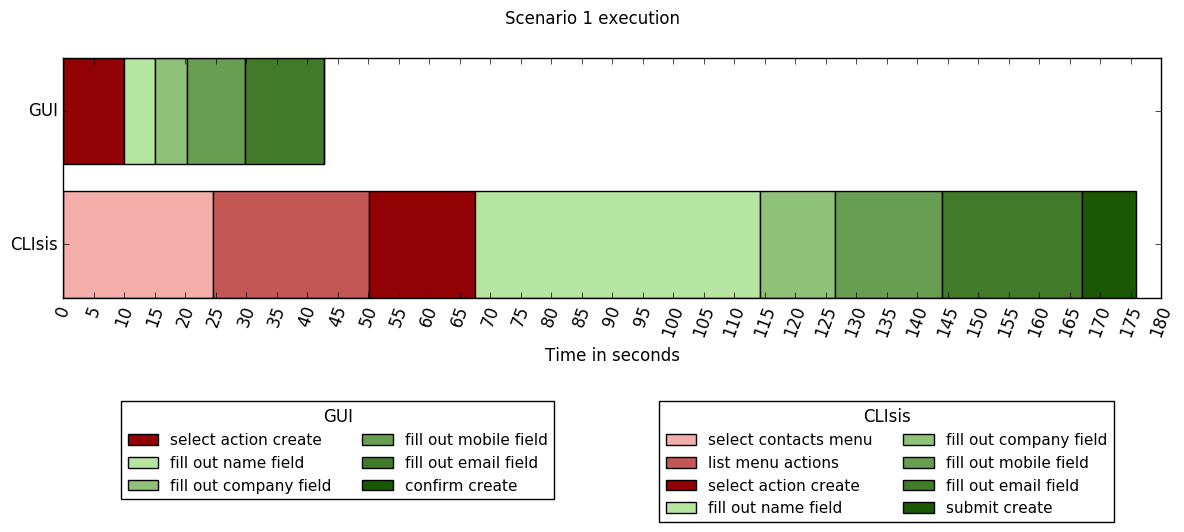
\includegraphics[width=\textwidth]{figures/scenario1}
	\caption{Red shades: invoke action create, green shades: fill out create parameters}
	\label{figure:scenario1timetrial}
\end{figure}

\subsubsection{Scenario 2}
For scenario 2, the measured time is 49.35 seconds in the \acrshort{gui} and 175.16 seconds in CLIsis, which equals to a measured increase of about 355\%.

\begin{figure}[H]
	\center
	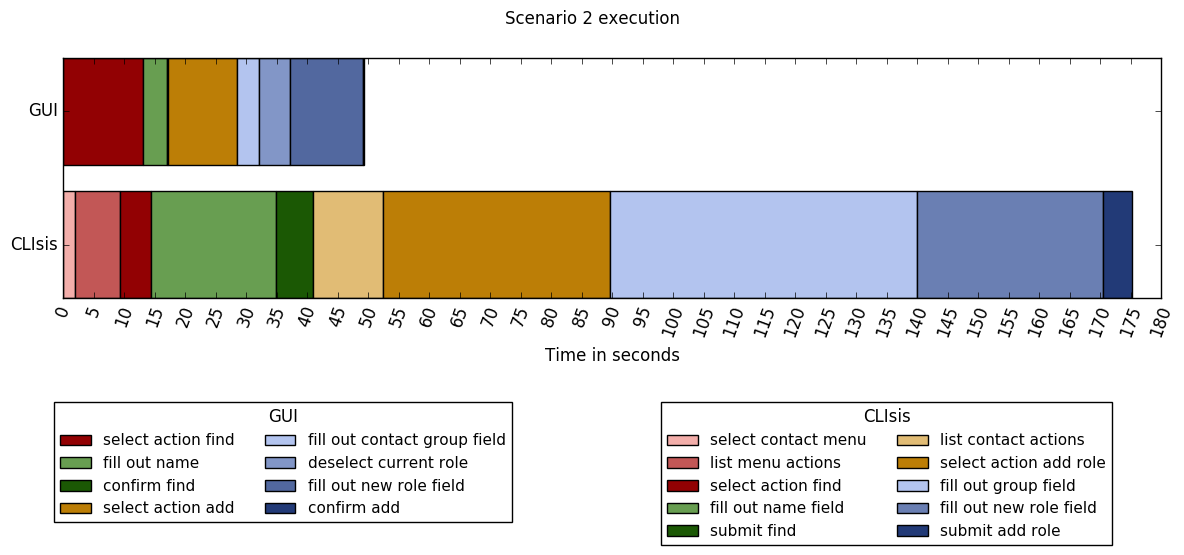
\includegraphics[width=\textwidth]{figures/scenario2}
	\caption{Red shades: invoke action find, green shades: fill out create parameters, yellow shades: invoke action add, blue shades: fill out add parameters}
	\label{figure:scenario2timetrial}
\end{figure}

\subsubsection{Scenario 3}
For scenario 3, the measured time is 31.94 seconds in the \acrshort{gui} and 127.33 seconds in CLIsis, which equals to a measured increase of about 399\%.

\begin{figure}[H]
	\center
	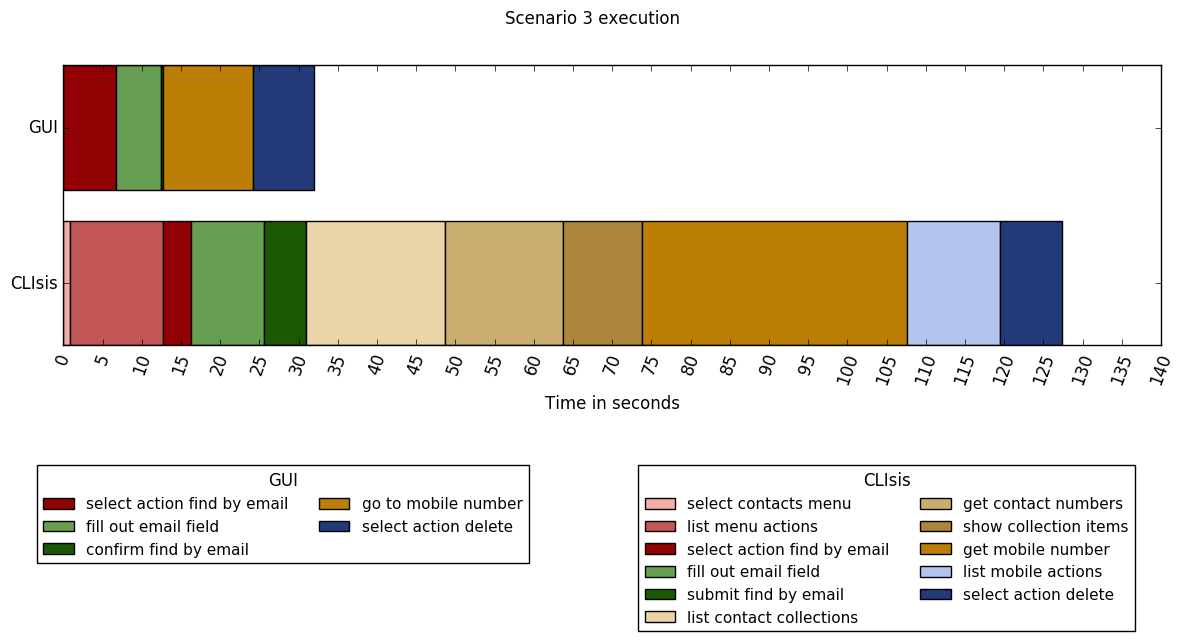
\includegraphics[width=\textwidth]{figures/scenario3}
	\caption{Red shades: invoke action find by email, green shades: fill out find by email parameters, yellow shades: go to mobile number, blue shades: invoke action delete}
	\label{figure:scenario3timetrial}
\end{figure}

\subsubsection{Scenario 4}
For scenario 4, the measured time is 40.54 seconds in the \acrshort{gui} and 161.51 seconds in CLIsis, which equals to a measured increase of about 398\%.

\begin{figure}[H]
	\center
	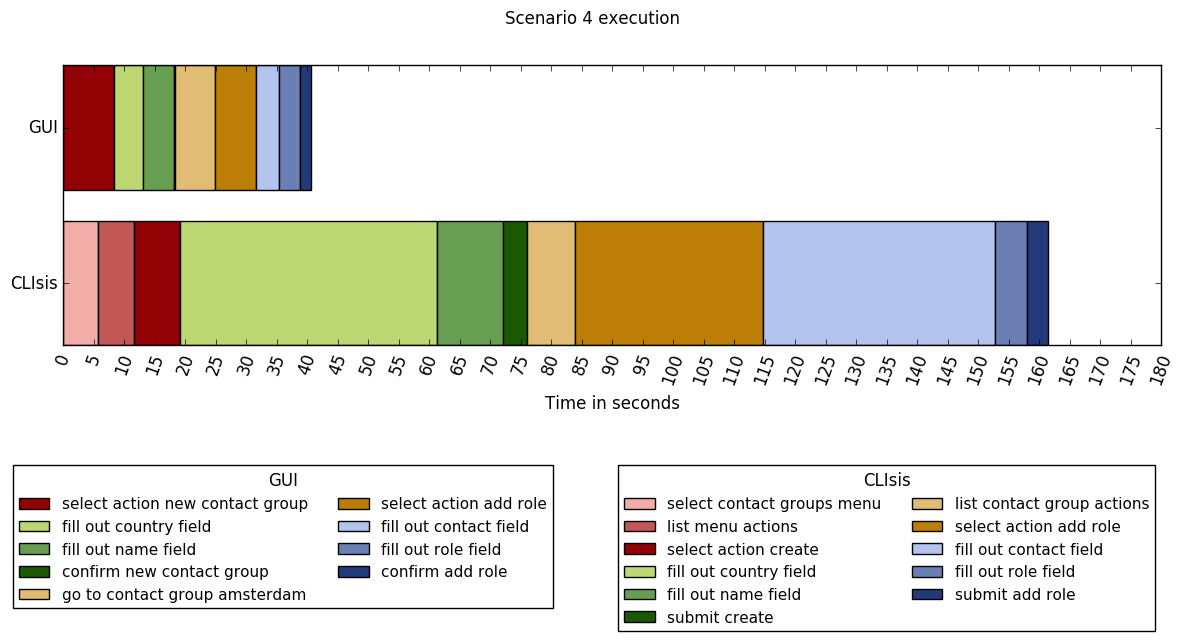
\includegraphics[width=\textwidth]{figures/scenario4}
	\caption{Red shades: invoke action create contact group, green shades: fill out create parameters, yellow shades: invoke action add role, blue shades: fill out add role parameters}
	\label{figure:scenario4timetrial}
\end{figure}

\subsubsection{Scenario 5}
For scenario 5, the measured time is 38.68 seconds in the \acrshort{gui} and 213.22 seconds in CLIsis, which equals to a measured increase of about 551\%.

\begin{figure}[H]
	\center
	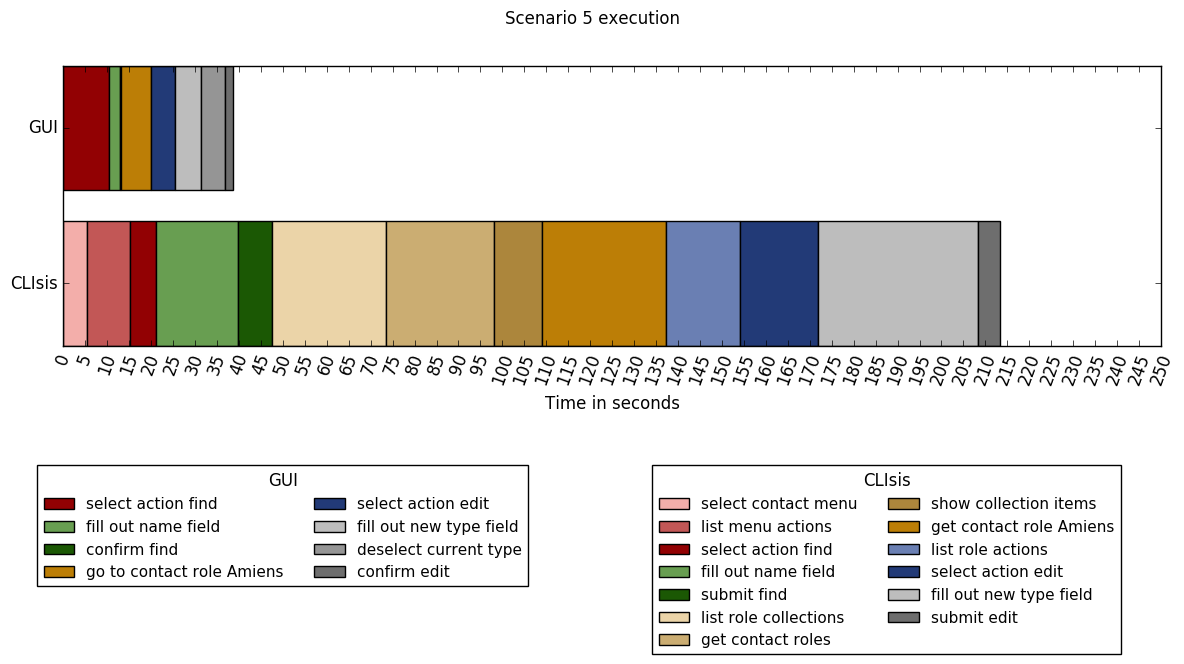
\includegraphics[width=\textwidth]{figures/scenario5}
	\caption{Red shades: invoke action find, green shades: fill out find parameters, yellow shades: get contact role, blue shades: invoke action edit, grey shades: fill out edit parameters}
	\label{figure:scenario5timetrial}
\end{figure}

\subsection{Performance difference}
\label{subsection:performancedifference}
With both a theoretical and empirical approach, we can now compare the results to see how accurate the \acrshort{goms} analyses were. Table~\ref{table:gomstimetrialcomparison} shows the difference between the empirical data and the predicted \acrshort{goms} data. On average, the empirical measurements were around 15\% higher than the predicted times for the \acrshort{gui}, whereas for CLIsis, the average increase in execution time compared to the predicted time was around 57\%. This can be attributed to a number of reasons, but the most likely reason is the learning curve of the new user interface. As stated in section~\ref{subsection:timetrial_evaluation}, the order in which the test subjects performed the tasks in CLIsis was S1, S5, S2, S4, S3. If we now look at the difference for CLIsis in that order, we see that the difference between empirical and predicted data is consistently decreasing: +91\%, +69\%, +64\%, +36\% and +25\%. Considering the very limited amount of time the users spent working with CLIsis yet showing a strong improvement in performance already, it is likely that once a user has more experience with CLIsis their performance will increase significantly. In addition, it is inevitable that the test subjects were familiar with \acrshortpl{gui} and thus felt more familiar with the graphical interface. This clarifies the smaller difference between the predicted and empirical data for the \acrshort{gui}. \todo{Heel goed geanalyseerd! Duidelijk!}

The timelines in section~\ref{subsection:timetrial_evaluation} reveal that filling out parameter fields are a major reason for the strong increase in execution time in CLIsis as compared to the \acrshort{gui}. Upon inspection of some of these parameters, it becomes clear that the equivalent of a dropdown menu in the \acrshort{gui} causes a great increase in execution time, as all options in the dropdown menu are exposed in the \acrshort{rest} API as the 'choices' of a parameter. In the new user interface, the speech synthesiser will name all of these choices, causing a delay just by the amount of speech alone. This is illustrated in figure~\ref{figure:parametercomparison}. There's also the issue of receiving too much information in one go, requiring users to reinvoke the action to hear the options again, increasing the delay even more.

That said, nothing obliges the user to let the speech synthesiser finish speaking. Once the user gets more accustomed with the user interface, the speech function will serve more as a reminder rather than a requirement. The \acrshort{goms} analyses all assume completion of every sentence, so in theory, execution times could fall below predicted times with experienced users. This is particularly realistic for routine tasks.

\begin{table}[h]
	\center
	
	\begin{tabular}{lllllll}
		\toprule
		Scenario		&	GOMS$_{\text{GUI}}$	& Time trial$_{\text{GUI}}$	& Diff. & GOMS$_{\text{CLIsis}}$	& Time trial$_{\text{CLIsis}}$	& Diff. \\		
		\midrule
		1	&	38.46s						& 42.80s							& +11\%					& 92.20s						& 175.87s							& +91\% \\
		2	& 38.24s						& 49.35s							& +29\%					& 106.96s					& 175.16s							& +64\% \\
		3	& 23.10s						& 31.94s							& +38\%					& 101.76s					& 127.33s							&	+25\%\\
		4	& 45.32s						& 40.54s							& -11\%					& 118.92s					& 161.51s							&	+36\%\\
		5	& 39.54s						& 38.68s							& -2\%						& 125.88s					& 213.22s							& +69\%\\
		\bottomrule
	\end{tabular}
	\caption{A comparison of the \acrshort{goms} and time trial results}
	\label{table:gomstimetrialcomparison}
\end{table}
\todo{Suggestion: add here the term "predicted" in the table caption}

\begin{figure}[h]
	\center
	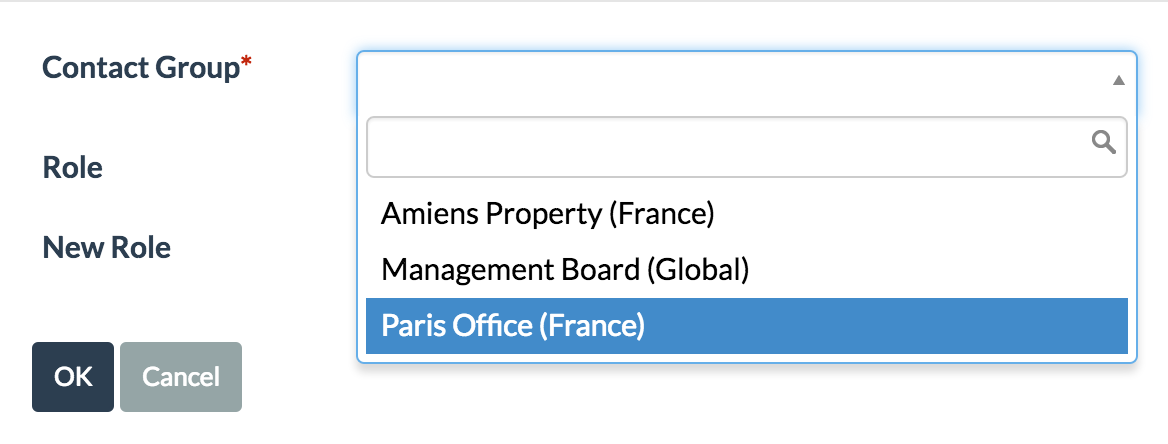
\includegraphics[width=0.49\textwidth]{figures/paramsgui}
	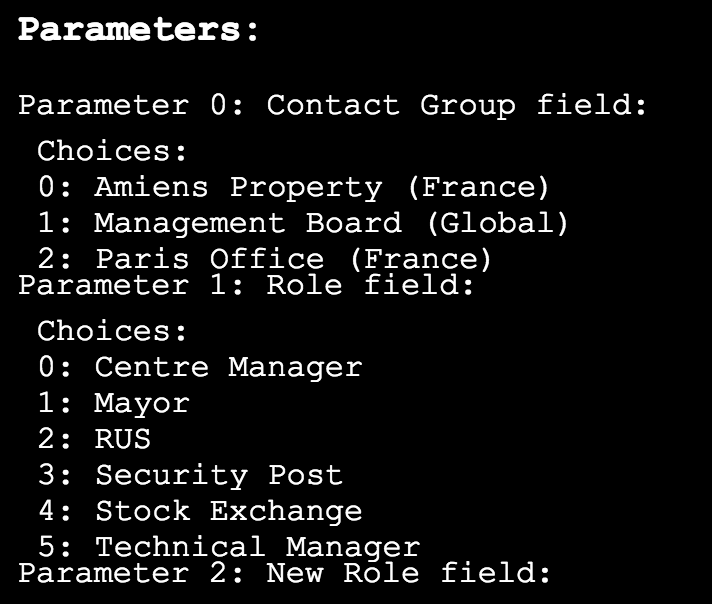
\includegraphics[scale=.5]{figures/paramsclisis}
	\caption{A comparison between the display of parameters in the GUI and CLIsis}
	\label{figure:parametercomparison}
\end{figure}